\documentclass[UTF8]{article}
\usepackage{graphicx}
\usepackage{ctex}
\usepackage{amsmath}
\usepackage{amsfonts}
\usepackage{amssymb}
\usepackage{enumerate}
\usepackage{color}
\usepackage{setspace}
\usepackage{pythonhighlight}
\usepackage{bm}

\usepackage
[a4paper,
text={146.4true mm,239.2 true mm},
top= 26.2true mm,
left=31.8 true mm,
head=6true mm,
headsep=6.5true mm,
foot=16.5true mm]
{geometry} % 设置文本的边距
\input{../setup/format}

\begin{document}
\title{Homework 4 of Stochastic Processes}
\author{姓名:林奇峰\qquad 学号:19110977}
\maketitle

\section{Exercise 2.23}
\begin{figure}[h]
    \centering
    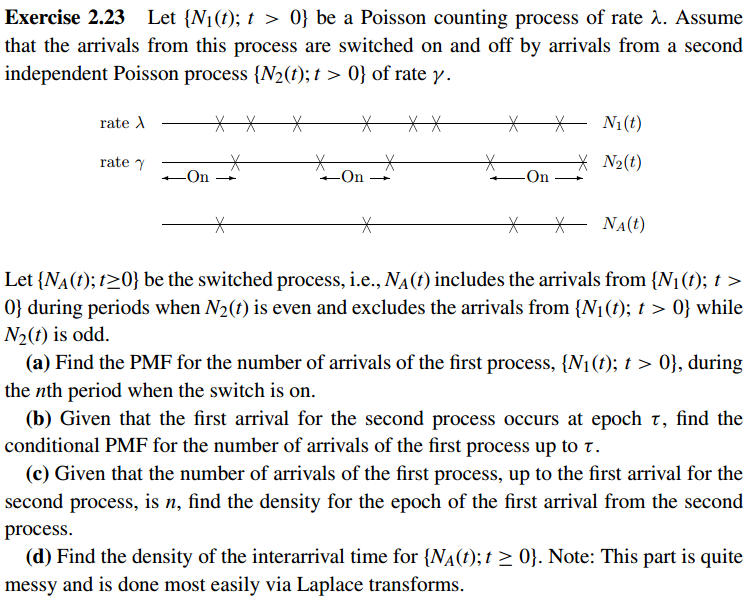
\includegraphics[width=5.5in]{exercise__2_23.png}
\end{figure}
\textbf{Soultions}

    \begin{enumerate}[a)]
        \item The combined process $\{N_1(t)+N_2(t)\}$ is also a Poisson process with rate $\lambda+\gamma$. During the $n$th period when the switch is on, once there is an arrival of process $\{N_2(t);t>0\}$, the $n$th period will end. Therefore, the PMF for the number of arrivals of the first process $\{N_1(t);t>0\}$ is
        \begin{equation*}
            \text{p}_{N_1(t)}(k)=\big(\frac{\lambda}{\lambda+\gamma}\big)^k\frac{\gamma}{\lambda+\gamma}
        \end{equation*}
        where $k$ denotes the number of arrivals of the first process $\{N_1(t);t>0\}$ and $n$ denotes the $n$th period when the switch is on.
        \item According to the Theorem 2.2.10, \textsl{for a Poisson of rate $\lambda$, and for any $t>0$, the PMF for $N(t)$, i.e., the number of arrivals in $(0,t]$, is given by the Poisson PMF,}
        \begin{equation*}
            \text{p}_{N(t)}(n)=\frac{(\lambda t)^n\exp(-\lambda t)}{n!}.
        \end{equation*}
        Since $\{N_1(t);t>0\}$ and $\{N_2(t);t>0\}$ are independent,given that the first arrival for process $\{N_2(t);t>0\}$ at epoch $\tau$, the conditional PMF for the number of arrivals of $\{N_1(t);t>0\}$ up to $\tau$ is
        \begin{equation*}
            \text{p}_{N_1(\tau)}(n)=\frac{(\lambda\tau)^n\exp(-\lambda\tau)}{n!}.
        \end{equation*}
        \item Suupose that the first arrival of process $\{N_2(t);t>0\}$ is at epcoh $\tau$, according to the Bayes' Law, we can obtain that
        \begin{equation*}
            \text{p}_{N_1(\tau)}(n)\text{f}_{S^2_1|N_1(\tau)}(\tau|n)=\text{f}_{S^2_1}(\tau)\text{p}_{N_1(\tau)|S^2_1}(n|\tau)
        \end{equation*}
        where $S^2_1$ denotes the 1rd arrival of process 2. 
        
        From a) we can know that 
        \begin{equation*}
            \text{p}_{N_1(\tau)}(n)=\big(\frac{\lambda}{\lambda+\gamma}\big)^n\frac{\gamma}{\lambda+\gamma}
        \end{equation*}
        
        From b) we can know that
        \begin{equation*}
            \text{p}_{N_1(\tau)|S^2_1}(n|\tau)=\frac{(\lambda\tau)^n\exp(\lambda\tau)}{n!}
        \end{equation*}

        And from the equation (2.13) $\text{f}_{S_n}(t)=\frac{\lambda^n t^{n-1}\exp(-\lambda t)}{(n-1)!}$ in the textbook we can konw that
        \begin{equation*}
            \text{f}_{S^2_1}(\tau)=\gamma\exp(-\gamma\tau)
        \end{equation*}

        Therefore,
        \begin{equation*}
            \begin{aligned}
            \text{f}_{S^2_1|N_1(\tau)}(\tau|n)
            &=\text{f}_{S^2_1}(\tau)
            \frac{\text{p}_{N_1(\tau)|S^2_1}(n|\tau)}{\text{p}_{N_1(\tau)}(n)}\\
            &=\gamma e^{-\gamma\tau}\cdot\frac{(\lambda\tau)^n e^{-\lambda\tau}}{n!}\cdot\frac{(\lambda+\gamma)^{n+1}}{\lambda^n\gamma}\\
            &=\frac{(\lambda+\gamma)^{n+1}\tau^n e^{-(\lambda+\gamma)\tau}}{n!}
            \end{aligned}
        \end{equation*}
        \item 
        Since $N_1(t);t>0$ and $N_2(t);t>0$ are both independent and both renewal process, $N_A(t);t>0$ should be also a renewal process. Therefore, each interval of $N_A(t);t>0$ is independent and identically distributed.

        Let $X_A$ denote the interval of process $\{N_A(t);t\geq 0\}$, $X$ denote the interval of the combined process $\{N_1(t)+N_2(t);t>0\}$, and $X_2$ denote the interval of process $\{N_2(t);t>0\}$.

        There exists two cases:
        \begin{enumerate}[1.]
            \item If the next arrival belongs to process $\{N_1(t);t>0\}$, $X_A=X$
            \item If the next arrivals belongs to process $\{N_2(t);t>0\}$, then $X_A$ is the sum of three rv's: $X$, $X_2$ and $X_A$。
        \end{enumerate}

        Therefore, the density of the interarrival time for $\{N_A(t);t\geq 0\}$ is
        \begin{equation*}
            \begin{aligned}
                \text{f}_{X_A}(x)
                &=\frac{\lambda}{\lambda+\gamma}\text{f}_X(x)+(\frac{\gamma}{\lambda+\gamma}\text{f}_X(x))\otimes\text{f}_{X_2}(x)\otimes\text{f}_{X_A}(x)\\
                &=\frac{\lambda}{\lambda+\gamma}\cdot(\lambda+\gamma)e^{-(\lambda+\gamma)x}+[\frac{\gamma}{\lambda+\gamma}\cdot(\lambda+\gamma)e^{-(\lambda+\gamma)x}]\otimes(\gamma e^{-\gamma x})\otimes\text{f}_{X_A}(x)\\
                &=\lambda e^{-(\lambda+\gamma)x}+(\gamma e^{-(\lambda+\gamma)x})\otimes(\gamma e^{-\gamma x})\otimes\text{f}_{X_A}(x)
            \end{aligned}
        \end{equation*}
        where $\otimes$ denotes the convolution operator anbd all functions satisfy $f(x)=0$ for $x<0$.

        Let
        \begin{equation*}
            \begin{aligned}
                f_1(x)&=\lambda e^{-(\lambda+\gamma)x}\\
                f_2(x)&=\gamma e^{-(\lambda+\gamma)x}\\
                f_3(x)&=\gamma e^{-\gamma x}
            \end{aligned}
        \end{equation*}
        Then we can obtain that:
        \begin{equation*}
            \text{f}_{X_A}(x)=f_1(x)+f_2(x)\otimes f_3(x)\otimes\text{f}_{X_A}(x)
        \end{equation*}

        Apply the Laplace transforms
        \begin{equation*}
            \begin{aligned}
                \mathcal{L}[\text{f}_{X_A}]&=\mathcal{L}[f_1]+\mathcal{L}[f_2]\cdot\mathcal{L}[f_3]\cdot\mathcal{L}[\text{f}_{X_A}]\\
                &\Downarrow\\
                \mathcal{L}[\text{f}_{X_A}]&=\frac{\mathcal{L}[f_1]}{1-\mathcal{L}[f_2]\mathcal{L}[f_3]}
            \end{aligned}
        \end{equation*}

        Since
        \begin{equation*}
            \begin{aligned}
                \mathcal{L}[f_1]&=\int^\infty_0\lambda e^{-(\lambda+\gamma)t}\cdot e^{-st}dt&&=\frac{\lambda}{\lambda+\gamma+s}\\
                \mathcal{L}[f_2]&=\int^\infty_0\gamma e^{-(\lambda+\gamma)t}\cdot e^{-st}dt&&=\frac{\gamma}{\lambda+\gamma+s}\\
                \mathcal{L}[f_3]&=\int^\infty_0\gamma e^{-\gamma t}\cdot e^{-st}dt&&=\frac{\gamma}{\gamma+s}
            \end{aligned}
        \end{equation*}

        \begin{equation*}
            \begin{aligned}
                \mathcal{L}[\text{f}_{X_A}]&=\frac{\lambda}{\lambda+\gamma+s}\cdot\frac{1}{1-\frac{\gamma}{\lambda+\gamma+s}\cdot\frac{\gamma}{\gamma+s}}\\
                &=\frac{\lambda}{(\lambda+\gamma+s)-\frac{\gamma^2}{\gamma+s}}\\
                &=\frac{\lambda(\gamma+s)}{(\lambda+\gamma+s)(\gamma+s)-\gamma^2}\\
                &=\frac{\lambda(\gamma+s)}{\lambda\gamma+(\lambda+2\gamma)s+s^2}\\
                &=\frac{F_1(s)}{F_2(s)}
            \end{aligned}
        \end{equation*}

        To obatin $\text{f}_{X_A}$, it needs to perform inverse Laplace transforms.

        For $F_2(s)$, $(\lambda+2\gamma)^2-4\lambda\gamma=\lambda^2+4\gamma^2>0$ and it has two roots with real value. Then we can rewrite $F_2(s)$ as 
        \begin{equation*}
            \begin{aligned}
                F_2(s)=\bigg(s-\frac{-(\lambda+2\gamma)-\sqrt{\lambda^2+4\gamma^2}}{2}\bigg)\bigg(s-\frac{-(\lambda+2\gamma)+\sqrt{\lambda^2+4\gamma^2}}{2}\bigg)=(s-s_1)(s-s_2)
            \end{aligned}
        \end{equation*}

        And $\mathcal{L}[\text{f}_{X_A}]$ can be rewritten as
        \begin{equation*}
            \mathcal{L}[\text{f}_{X_A}]=\frac{k_1}{s-s_1}+\frac{k_2}{s-s_2}
        \end{equation*}
        
        The value of $k_1$ and $k_2$ can be solved by:
        \begin{equation*}
            \begin{aligned}
                k_1&=(s-s_1)\mathcal{L}[\text{f}_{X_A}]\big|_{s=s_1}\\
                &=\frac{\lambda(\gamma+s)}{s-s_2}\bigg|_{s=s_1}\\
                &=\frac{\lambda(\gamma+\frac{-(\lambda+2\gamma)-\sqrt{\lambda^2+4\gamma^2}}{2})}{\frac{-(\lambda+2\gamma)-\sqrt{\lambda^2+4\gamma^2}}{2}-\frac{-(\lambda+2\gamma)+\sqrt{\lambda^2+4\gamma^2}}{2}}\\
                &=\frac{\lambda\frac{-\lambda-\sqrt{\lambda^2+4\gamma^2}}{2}}{-\sqrt{\lambda^2+4\gamma^2}}\\
                &=\frac{\lambda(\lambda+\sqrt{\lambda^2+4\gamma^2})}{2\sqrt{\lambda^2+4\gamma^2}}\\
                &=\frac{\lambda}{2}\bigg(1+\frac{\lambda}{\sqrt{\lambda^2+4\gamma^2}}\bigg)\\
                k_2 &=(s-s_2)\mathcal{L}[\text{f}_{X_A}]\big|_{s=s_2}\\
                &=\frac{\lambda(\gamma+s)}{s-s_1}\bigg|_{s=s_2}\\
                &=\frac{\lambda(\gamma+\frac{-(\lambda+2\gamma)+\sqrt{\lambda^2+4\gamma^2}}{2})}{\frac{-(\lambda+2\gamma)+\sqrt{\lambda^2+4\gamma^2}}{2}-\frac{-(\lambda+2\gamma)-\sqrt{\lambda^2+4\gamma^2}}{2}}\\
                &=\frac{\lambda\frac{-\lambda+\sqrt{\lambda^2+4\gamma^2}}{2}}{\sqrt{\lambda^2+4\gamma^2}}\\
                &=\frac{\lambda(-\lambda+\sqrt{\lambda^2+4\gamma^2})}{2\sqrt{\lambda^2+4\gamma^2}}\\
                &=\frac{\lambda}{2}\bigg(1-\frac{\lambda}{\sqrt{\lambda^2+4\gamma^2}}\bigg)
            \end{aligned}
        \end{equation*}

        According to the formula of inverse Laplace tranform:
        \begin{equation*}
            f(t)=\mathcal{L}^{-1}[F(s)]=\mathcal{L}^{-1}[\frac{k_1}{s-s_1}+\frac{k_2}{s-s_2}+\cdots+\frac{k_n}{s-s_n}]=\sum_{i=1}^nk_ie^{s_it}
        \end{equation*}

        we can obtain $\text{f}_{X_A}$ as
        \begin{equation*}
            \begin{aligned}
                \text{f}_{X_A}(x)&=k_1\cdot e^{\frac{-(\lambda+2\gamma)-\sqrt{\lambda^2+4\gamma^2}}{2}x}+k_2\cdot e^{\frac{-(\lambda+2\gamma)+\sqrt{\lambda^2+4\gamma^2}}{2}x}\\
                &=k_1\cdot\exp\bigg[\frac{-(\lambda+2\gamma)-\sqrt{\lambda^2+4\gamma^2}}{2}x\bigg]+k_2\cdot\exp\bigg[\frac{-(\lambda+2\gamma)+\sqrt{\lambda^2+4\gamma^2}}{2}x\bigg]
            \end{aligned}
        \end{equation*}
    \end{enumerate}

    
\section{Exercise 2.25}
\begin{figure}[h]
    \centering
    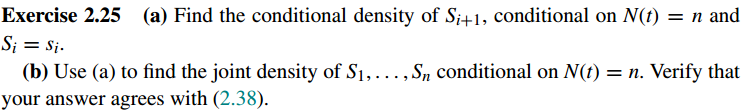
\includegraphics[width=5.5in]{exercise_2_25.png}
\end{figure}
\textbf{Solutions}
\begin{enumerate}[a)]
    \item From the equation (2.41) in the textbook,
        \begin{equation*}
            \text{Pr}\{S_1>\tau|N(t)=n\}=\bigg[\frac{t-\tau}{t}\bigg]^n\qquad\text{for $0<\tau\leq t$}
        \end{equation*}
        we can obtain that
        \begin{equation*}
            \begin{aligned}
                \text{f}_{S_1|N(t)}(\tau|n)
                &=(1-\text{Pr}\{S_1>\tau|N(t)=n\})'\\
                &=\bigg(1-\bigg[\frac{t-\tau}{t}\bigg]^n\bigg)'\\
                &=-n\cdot\bigg[\frac{t-\tau}{t}\bigg]^{n-1}\cdot-\frac{1}{t}\\
                &=\frac{n(t-\tau)^{n-1}}{t^n}
            \end{aligned}           
        \end{equation*}

        Then, given that $N(t)=n$ and $S_i=s_i$, we can obtain that
        \begin{equation*}
            \begin{aligned}
                \text{f}_{S_{i+1}|N(t),S_i}(s_{i+1}|n,s_i)
                &=\text{f}_{X_{i+1}|N(t),S_i}(s_{i+1}-s_i|n,s_i)\\
                &=\text{f}_{X_{i+1}}|\widetilde{N}(s_i,t)(s_{i+1}-s_i|n-i)\\
                &=\frac{(n-i)[t-s_i-(s-{i+1}-s_i)]^{n-i-1}}{(t-s_i)^{n-i}}\\
                &=\frac{(n-i)(t-s_{i+1})^{n-i-1}}{(t-s_i)^{n-i}}
            \end{aligned}
        \end{equation*}
    \item For $S_i$, the conditional probability is independent of $S_1,S_2,\dots,S_{i-2}$, and thus
        \begin{equation*}
            \begin{aligned}
                \text{f}_{S^{(n)}|N(t)=n}(s^{(n)}|n)
                &=\text{f}_{S_1|N(t)}\cdot\text{f}_{S_2|N(t),S_1}\cdots\text{f}_{S_n|N(t),\dots,S_{n-1}}\\
                &=\text{f}_{S_1|N(t)}\cdot\text{f}_{S_2|N(t),S_1}\cdots\text{f}_{S_n|N(t),S_{n-1}}\\
                &=\frac{n(t-s_1)^{n-1}}{t^n}\cdot\frac{(n-1)(t-s_2)^{n-2}}{(t-s_1)^{n-1}}\cdots\frac{(t-s_n)^0}{t-s_{n-1}}\\
                &=\frac{n!}{t^n}
            \end{aligned}
        \end{equation*}
\end{enumerate}

\end{document}